\documentclass[a4paper,10pt, notitlepage]{report}
\usepackage{geometry}
\geometry{verbose,tmargin=30mm,bmargin=25mm,lmargin=25mm,rmargin=25mm}

\usepackage[utf8]{inputenc}
\usepackage[sectionbib]{natbib}
\usepackage{url, hyperref}

\usepackage{amssymb}
\usepackage{amsmath}
\usepackage{amsthm}
\usepackage{mathtools}
\usepackage{bbm}

\usepackage{enumitem}
\usepackage{xcolor}
\usepackage{cancel}
\usepackage{float}

\PassOptionsToPackage{hyphens}{url}
\hypersetup{colorlinks=true,citecolor=blue}

\newtheorem{thm}{Theorem}
\newtheorem{lemma}[thm]{Lemma}
\newtheorem{proposition}[thm]{Proposition}
\newtheorem{remark}[thm]{Remark}
\newtheorem{defn}[thm]{Definition}

\theoremstyle{plain}
\newtheorem*{exercise*}{Exercise}
\newtheorem{exercise}{Exercise}


%%%%%%%%%%%%%%%%%%%% Notation stuff
\newcommand{\pr}{\operatorname{Pr}} %% probability
\newcommand{\var}{\operatorname{Var}} %% variance
\newcommand{\ev}{\operatorname{\mathbb{E}}}
\newcommand{\rs}{X_1, X_2, \ldots, X_n} %%  random sample
\newcommand{\irs}{X_1, X_2, \ldots} %% infinite random sample
\newcommand{\rsd}{x_1, x_2, \ldots, x_n} %%  random sample, realized
\newcommand{\bX}{\boldsymbol{X}} %%  random sample, contracted form (bold)
\newcommand{\bx}{\boldsymbol{x}} %%  random sample, realized, contracted form (bold)
\newcommand{\bT}{\boldsymbol{T}} %%  Statistic, vector form (bold)
\newcommand{\bt}{\boldsymbol{t}} %%  Statistic, realized, vector form (bold)
\newcommand{\emv}{\hat{\theta}}
\DeclarePairedDelimiter\ceil{\lceil}{\rceil}
\DeclarePairedDelimiter\floor{\lfloor}{\rfloor}

\newcommand{\R}{\mathbb{R}}

% Title Page
\title{Exercise Cauchy Location Posterior }
\author{Class: Bayesian Statistics \\ Instructor: Luiz Max Carvalho \\ Student: Lucas Machado Moschen}
\date{\today}

\begin{document}
\maketitle

\textbf{Turn in date: until 05/26/2021 at 23:59h Brasilia Time.}

\begin{center}
\fbox{
    \fbox{
        \parbox{0.95\textwidth}{
    \begin{exercise*}
        Take $X_i \sim \operatorname{Cauchy}(\theta, 1)$, $i = 1, 2,\ldots, 10$.
        In particular, suppose 
        \begin{equation}
            \label{eq:data}
            \boldsymbol{x} = \{-5, -3, 0, 2, 4, 5, 7, 9, 11, 14\}.
        \end{equation}
        \begin{itemize}
        \item[i)] Compute the MLE and $l^{\prime\prime}$;
        \item[ii)] Deduce the parameters of the normal approximation to $p(\theta \mid \boldsymbol{x})$;
        \item[iii)] Use an MCMC routine to sample from $p(\theta \mid \boldsymbol{x})$, obtain a posterior approximation to its density and compare it to the normal approximation;
        \item[iv)] Simulate data sets of sizes 
        $$n=20, 50, 100, 500, 1000 \text{ and } 10, 000$$ and repeat iii.
        \item[v)] See if you can reduce/increase the discrepancy between the posterior and its approximation by fiddling with the prior (without breaking the regularity assumptions!).
        \end{itemize}  
    \end{exercise*}  
        }
    }
}
\end{center}

\section*{Maximum likelihood estimator}

The probability density function of the Cauchy distribution with location
parameter $\theta$ and scale parameter $\gamma=1$ with respect to the Lebesgue
measure is 
    \begin{equation}
        \label{eq:pdf-cauchy}
        f(x|\theta) = \frac{1}{\pi[1 + (x - \theta)^2]}.
    \end{equation} 
    Starting from that, we can define the likelihood for a sample (i.i.d.)
    with size n
    \begin{equation}
        \label{eq:likelihood-cauchy}
        L(\theta|\bx) = \prod_{i=1}^{n} f(x_i|\theta) = \left[\pi^{n}\prod_{i=1}^{n}[1 + (x_i - \theta)^2]\right]^{-1}
    \end{equation}
    and the log-likelihood
    \begin{equation}
        \label{eq:loglikelihood-cauchy}
        l(\theta|\bx) = -n\log(\pi) - \sum_{i=1}^{n}\log\left(1 + (x_i - \theta)^2\right).
    \end{equation}
    We shall prove this function has an global maximum. To do this, we will
    first prove that $-l(\theta|\bx)$ is a coercive function, that is, for each
    sequence $\{\theta_n\}_{n\in\mathbb{N}}$, such that $|\theta_n| \to +
    \infty$, we have that $-l(\theta|\bx) \to \infty$. By triangular
    inequality, for $i=1,...,n$,
    $$|x_i - \theta| \ge |\theta| - |x_i| \implies 1 + |x_i - \theta|^2 \ge
    1 + (|\theta| - |x_i|)^2 \implies \log(1 + |x_i - \theta|^2) \ge
    \log(1 + (|\theta| - |x_i|)^2)$$
    if $|\theta| > |x_i|$.  Therefore, if $|\theta_n| \to + \infty$, taking
    $n$ largely enough, by the relation above, 
    $$
    \log(1 + |x_i - \theta|^2) \to + \infty,
    $$
    what proves that $-l(\theta|\bx)$ is coercive. Given that it is continuos,
    we know there is a global minimum $\bar{\theta}$ \cite[Corolary
    1.2.8]{otimizacao}, and $l(\theta|\bx)$ has a global maximum. 
    In order to find the maximum likelihood estimator (MLE) $\hat{\theta}(\bx)$, we find the
    stationary points for the unrestricted problem: 
    \begin{equation}
        \label{eq:derivarive-log-cauchy}
        \frac{d}{d\theta}l(\theta|\bx) = 2\sum_{i=1}^{n} \frac{x_i-\theta}{1 + (x_i - \theta)^2} = 0.
    \end{equation}
    A numerical procedure must be used to solve
    \ref{eq:derivarive-log-cauchy}. We search the
    solution in the interval 
    $$I = (\min\{x_i\}_{i=1}^{n}, \max\{x_i\}_{i=1}^{n}),$$
    because taking $i=1,...,n$, 
    \begin{itemize}
        \item if $\theta = \min\{x_i\}_{i=1}^{n}, x_i -
        \theta \ge 0$ and $l'(\theta|\bx) \ge 0$;
        \item if $\theta =
        \max\{x_i\}_{i=1}^{n}, x_i - \theta \le 0$ and $l'(\theta|\bx) \le 0$.
    \end{itemize} 
    what implies the existence of $\theta^* \in I$ such that $l'(\theta^*|\bx)
    = 0$, by the Intermediate Value Theorem \cite[Theorem 12, Page 184]{Lages1976}. We use the Brent’s method \cite{brent} to solve the problem and its
    implementation in SciPy \cite{2020SciPy-NMeth}. The codes are available at
    Github XXX. When $n=10$ and the data is \ref{eq:data}, teh solution is
    $$
    \hat{\theta}(\bx) \approx 4.531
    $$
    and the function can is drawn in Figure \ref{fig:log-likelihood-cauchy}
    \begin{figure}[!hb]
        \centering
        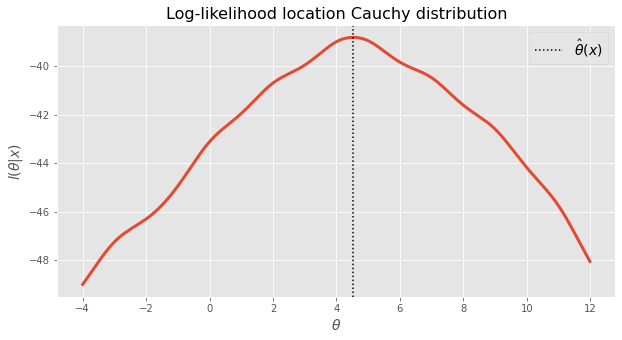
\includegraphics[width=0.8\textwidth]{../../images/log-likelihood.png}
        \caption{Log-likelihood of the parameter of location from the Cauchy distribution and MLE.}
        \label{fig:log-likelihood-cauchy}
    \end{figure}
    
    
    We differentiate once more 
    \begin{equation}
        \label{eq:dderivarive-log-cauchy}
        \frac{d^2}{d\theta^2}l(\theta|\bx) = 2\sum_{i=1}^{n} \frac{- 1 - (x_i - \theta)^2 + 2(x_i-\theta)^2}{(1 + (x_i - \theta)^2)^2} = 2\sum_{i=1}^{n} \frac{(x_i - \theta)^2-1}{( (x_i - \theta)^2+1)^2}
    \end{equation}
    and we obtain $l''$. We can test if the MLE is really the maximizer, that is,
    $l''\left(\hat{\theta}(\bx)\right) < 0$. In fact,
    $$
    l''\left(\hat{\theta}(\bx)\right) = -1.231 < 0.
    $$

\section*{Fisher information}

The fisher information for one observation is defined as
\begin{equation}
    \label{eq:fisher-info}
    I(\theta) = -\ev_{\theta}\left[\frac{d^2}{d\theta^2}l(\theta|x)\right] = -2\ev_{\theta}\left[\frac{(x - \theta)^2 - 1}{((x - \theta)^2 + 1)^2}\right].
\end{equation}

Therefore 
\begin{equation}
    \label{eq:ficher-cauchy-p1}
    \begin{split}
        I(\theta) &= 2\ev_{\theta}\left[\frac{1}{((x - \theta)^2 + 1)^2} - \frac{(x - \theta)^2}{((x - \theta)^2 + 1)^2}\right] \\
        &= 2\ev_{\theta}\left[\frac{1}{(x - \theta)^2 + 1} - \frac{2(x - \theta)^2}{((x - \theta)^2 + 1)^2}\right] \\
        &= 2\int_{\R} \frac{1}{\pi((x - \theta)^2 + 1)^2} - \frac{2(x - \theta)^2}{\pi((x - \theta)^2 + 1)^3} \, dx, [y = x - \theta, dy = dx] \\
        &= \frac{2}{\pi}\int_{\R} \frac{1}{(y^2 + 1)^2} - \frac{2y^2}{(y^2 + 1)^3} \, dy. \\
    \end{split}
\end{equation}

We have that 
$$
- \frac{2y^2}{(y^2 + 1)^3} = \frac{A}{(y^2+1)^3} + \frac{B}{(y^2+1)^2} \implies A + B(y^2 + 1) = -2y^2 \implies B = -2, A = 2.
$$
Then, 
\begin{equation}
    \label{eq:ficher-cauchy-p2}
    \begin{split}
        I(\theta) &= \frac{2}{\pi}\int_{\R} \frac{1}{(y^2 + 1)^2} - \frac{2y^2}{(y^2 + 1)^3} \, dy, \\
        &= \frac{2}{\pi}\int_{\R} \frac{1}{(y^2 + 1)^2} - \frac{2}{(y^2 + 1)^2} + \frac{2}{(y^2 + 1)^3} \, dy, \\ 
        &= \frac{2}{\pi}\int_{\R} \frac{-1}{(y^2 + 1)^2} + \frac{2}{(y^2 + 1)^3} \, dy, \\ 
        &= \frac{2}{\pi}(-S_2 + 2S_3),
    \end{split}
\end{equation}
where
$$
S_k = \int_{\R} \frac{1}{(y^2 + 1)^k} \, dy.
$$
Integrating by parts, we obtain 
$$
\int_{\R} \frac{1}{(y^2 + 1)^k} \,dy = \frac{y}{(y^2 + 1)^k}\bigg|_{-\infty}^{\infty} + \int_{\R} \frac{2ky^2}{(y^2 + 1)^{k+1}} \, dy = \int_{\R} \frac{2k}{(y^2 + 1)^k} - \frac{2k}{(y^2 + 1)^{k+1}} \, dy, 
$$
since the first expression is 0 whenever $k > 1/2$ and the second is
calculated in the same way as before. We conclude that 
$$
S_k =2k S_k - 2k S_{k+1} \implies S_{k+1} = \frac{2k - 1}{2k}S_k,
$$
where $k \ge 1$ and $S_1 = \arctan(y)\big|_{-\infty}^{\infty} = \pi$.
Following this, we obtain that 
$$
S_2 = \frac{1}{2}\pi \text{ and }S_3 = \frac{3}{4}\frac{1}{2}\pi = \frac{3}{8}\pi.
$$
The Fisher Information for one observation for the location parameter of the
Cauchy distribution is
\begin{equation}
    \label{eq:fisher-cauchy}
    I(\theta) = \frac{2}{\pi}\left({-\frac{1}{2}\pi + \frac{3}{4}\pi}\right) = \frac{1}{2}.
\end{equation}
For $n$ observations, 
\begin{equation}
    \label{eq:fisher-cauchy-n}
    I_n(\theta) = -\ev_{\theta}\left[\frac{d^2}{d\theta^2}l(\theta|\bx)\right] = -\ev_{\theta}\left[\frac{d^2}{d\theta^2}\sum_{i=1}^n l(\theta|x_i)\right] = \sum_{i=1}^n -\ev_{\theta}\left[\frac{d^2}{d\theta^2}l(\theta|x_i)\right] = nI(\theta) = \frac{n}{2}.
\end{equation}

\section*{General Regularity Conditions}

Here we shall verify if there is mathematical support for the convergence to
the Normal distribution of the posteriori. In order to do that, we shall first
verify the General Regularity Conditions \cite[Page 436]{schervish1996theory}.
The first four points are straightforward: 

\begin{enumerate}
    \item[1.] The parameter space is $\Omega = \R$, then it is finite.  
    \item[2.] Since $\Omega$ is an open set, its interior is itself.
    Therefore, $\theta \in \Omega = \text{int } \Omega$.   
    \item[3.] We will elicit the priors in the next section, with support
    on $\Omega$ and continuos everywhere.
    \item[4.] The log-likelihood, equation \ref{eq:loglikelihood-cauchy}, 
    is infinitely differentiable in $\R$ because it is a composition of
    infinitely differentiable functions and it is defined everywhere. The
    second derivative is explicit in equation
    \ref{eq:dderivarive-log-cauchy} and it is clearly continuos. 
\end{enumerate}

Although in this example the MLE is unique and the unique local maximum, this
is not always the case.  For instance, consider an example from \cite[Page 122]{young_smith_2005} where we have $X_1$ and $X_2$ iid distributed
from $Cauchy(\theta,1)$. Let $X_1 = a$ and $X_2 = b$. Therefore, a local maximum is solution to the
equation 
$$
\frac{a - \theta}{1 + (a - \theta)^2} + \frac{b - \theta}{1 + (b - \theta)^2} = 0,
$$
as we indicated in equation \ref{eq:derivarive-log-cauchy}. Simplifying the
system and factoring, we obtain 
$$
(a + b - 2\theta)(\theta^2 - (a + b)\theta + 1 + ab) = 0.
$$
If $\Delta = (a+b)^2 - 4(1 + ab) = (a - b)^2 - 4 > 0$, that is, $|X_1 - X_2|
> 2$, we have three solutions, 
$$
\theta_m = \frac{X_1 + X_2}{2}
$$
and the solutions of the polynomial of second order. The bad news is that, if
$\theta_1$ and $\theta_2$ are the solutions, 
$$
\frac{\theta_1 + \theta_2}{2} = \frac{X_1 + X_2}{2} = \theta_m
$$
and 
$$l''(\theta_m|X_1, X_2) = \frac{1}{2}\frac{(X_1 - X_2)^2 - 4}{((X_1 -
\theta_m)^2 + 1)^2} + \frac{1}{2}\frac{(X_1 - X_2)^2 - 4}{((X_2 -
\theta_m)^2 + 1)^2} > 0
$$
what implies we have a local minimum here. By the expression's symmetry \ref{eq:loglikelihood-cauchy}, we conclude that we have two possible values for the MLE with positive probability. According to \cite{young_smith_2005}, this problem appears with positive probability when $n$ tends to infinity. This problem complicates the demonstration of consistency of the MLE, but \cite{consistency-mle} proves that $\hat{\theta}(\bx)$ converges to the true value $\theta_0$ exponentially. By the continuity $l''(\cdot|x)$, the consistency of the MLE and the Continuos mapping theorem, we know that 
$$
l''(\hat{\theta}(\bx)|\bx) \overset{p}{\to} l''(\theta|\bx). 
$$
and
$$
l''^{-1}(\hat{\theta}(\bx)|\bx) \overset{p}{\to} l''^{-1}(\theta|\bx).
$$
However, we were not able to prove that 
$$
-l''^{-1}(\hat{\theta}(\bx)|\bx) \overset{p}{\to} 0.
$$
We believe this is the case because $-\ev[l''(\theta|\bx)] = \frac{n}{2} \to \infty$. We could not also prove the Conditions 6 and 7. The condition 6 can be seen similar to the consistency, so we also believe it is true. 

\section*{Normal approximation}

Following \cite[Theorem 7.89]{schervish1996theory}, let 
$$
\Sigma_n = -l''^{-1}(\hat{\theta}(\bx)|\bx)
$$
and the posterior density of $\Psi_n = \Sigma_n^{-1/2}(\theta - \hat{\theta}(\bx))$ converges (in probability uniformly on compact sets) to the standard Normal density. In other words, 
$$
\frac{\theta - \hat{\theta}(\bx)}{\Sigma_n^{1/2}} \sim \mathcal{N}(0,1)
$$
what implies that the parameters of the normal approximation are 
\begin{equation}
    \label{eq:mu-normal-approximation}
    \mu = \hat{\theta}(\bx) \approx 4.531
\end{equation}
and 
\begin{equation}
    \label{eq:sigma-normal-approximation}
    \sigma^2 = \Sigma_n \approx 1/1.231 \approx 0.812.
\end{equation}


\section*{Eliciting the priors}
\label{sec:priors}

In this section, we elicit two different priors to compare the results in the
next sections. 

\subsection*{Non-informative prior}

We use the Jeffreys' Prior which has the property of invariance to
reparametrization. Although this prior does not satisfy the likelihood
principle, it is good when no subjective information is given before the data.
We have already calculated the Fisher information before, then the prior is 
\begin{equation}
    \label{eq:jeffreys-prior}
    \pi(\theta) \propto I^{1/2}(\theta) \propto 1.
\end{equation}
We obtain a improper prior. Therefore, we need to prove the posterior is
proper almost surely.

The posterior will be 
$$
p(\theta|\bx) \propto f(\bx|\theta) \propto \prod_{i=1}^n \frac{1}{1 + (x_i - \theta)^2}
$$
Observe that, $\forall \theta \in \R$,
$$
0 < \frac{1}{1 + (x_i - \theta)^2} \le 1.
$$
Then, 
$$
\prod_{i=1}^n \frac{1}{1 + (x_i - \theta)^2} \le \frac{1}{1 + (x_1 - \theta)^2}
$$
and
$$
\int_{\Omega} \prod_{i=1}^n \frac{1}{1 + (x_i - \theta)^2} \, d\theta \le \int_{\Omega} \frac{1}{1 + (x_1 - \theta)^2} \, d\theta = \pi,
$$
what proves the posteriori is proper almost surely, even though its expression
is really difficult. 

\subsection*{Informative prior}

We already know that $\theta \in \R$ and we need a distribution over this space.
There are infinitely many options. We will consider two approaches. 

\subsubsection*{Maximum entropy prior}

Prior to the data, we have no knowledge about the position of the parameter.
In this approach, we define 
$$
\ev^{\pi}[\theta] = 0 \text{ and } \var^{\pi}[\theta] = \sigma^2
$$
and we use the Lebesgue measure as the reference measure $\pi_0(\theta)$. As
calculated in \cite[Example 3.2.4]{Robert2007}, the prior will have Normal
distribution with parameters $0$ and $\sigma^2$. We will compare small values
(strong prior) of $\sigma^2$ to large values (weak prior). In particular, we
will compare the values 
$$\sigma^2 = 1, 100 \text{ and }  10000.$$

\subsubsection*{Heavy tail prior}

The Normal distribution has a light tail and decreases exponentially to both
sides. It shall be interesting to analyse when the tail is heavier. We choose
the Cauchy distribution with location parameter 0 and scale parameter
$\gamma$. Here the mean and variance are undefined, so it's harder to compare
them with the Normal distribution with moment matching. However $\gamma$ is a scale parameter as $\sigma = \sqrt{\sigma^2}$ in
the Normal distribution. Therefore, we
will compare the values 
$$
\gamma = 1, 10 \text{ and } 100
$$
with the same interpretation as the Normal distribution. Figure
\ref{fig:comparison-priors} presents the comparison of the priors. 

\begin{figure}
    \centering
    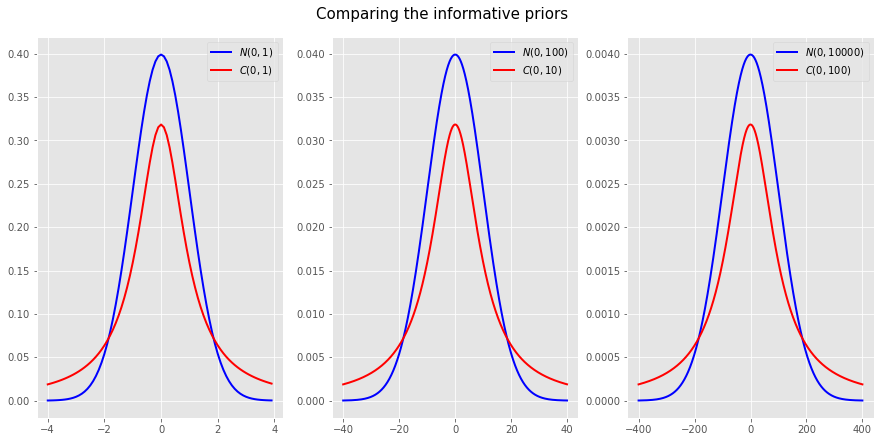
\includegraphics[width=0.9\textwidth]{../../images/priors-comparison.png}
    \caption{Comparing the distributions defined above.In blue, we see the Normal distribution, and in red we see the Cauchy distribution.}
    \label{fig:comparison-priors}
\end{figure}

\section*{Posterior distribution in the suggested case}

Considering the data given and the priors elicited previously, we can
obtain the posterior distribution through a MCMC routine. In this case, we use
PyMC3 library (\cite{pymc3}) in the Python language. We sampled from this
procedure 5000 draws and 1000 tune iterations. After simulating with each prior,
we get $\pr(\theta \ge 5 | X = \bx)$ and compare with the one given by
\cite{schervish1996theory}. The results are in the Table \ref{tb:table-prob}.
We can see that the most similar occurs when the prior is the lebesgue measure
in the real line and, for that reason, we can reproduce a similar figure. 

\begin{table}[ht]
    \centering
    \begin{tabular}{|c|c|c|c|c|c|c|c|}
        \hline
        \textbf{Prior}       & $U(-\infty, +\infty)$ & $\mathcal{N}(0,1)$ & $\mathcal{N}(0,100)$ & $\mathcal{N}(0,10000)$ & $C(0,1)$ & $C(0,10)$ & $C(0,100)$ \\ \hline
        \textbf{Probability} & 0.3569                & 0.0                  & 0.3251               & 0.3493                 & 0.1437   & 0.3022    & 0.3485      \\ \hline
        \end{tabular}
    \caption{Comparative among priors and its posteriors probabilities inferred.}
    \label{tb:table-prob}
\end{table}

Thereby, we can compare the posterior obtained by numerical integration with
the theoretical Normal distribution with mean and variance specified in equations
\ref{eq:mu-normal-approximation} and \ref{eq:sigma-normal-approximation}. The
comparison result can be seen in Figure
\ref{fig:comparison-normal-posteriori} and in Table \ref{tb:quantiles-probs}. The summary given by PyMC3 library is
in Table \ref{tb:mcmc-result}. We also plot the other posteriors generated by
the other priors in Figure \ref{fig:comparison-normal-posteriori-other}. 

\begin{table}[ht]
    \centering
    \begin{tabular}{|c|c|c|c|c|c|c|c|c|c|c|c|}
        \hline
         & \multicolumn{4}{c|}{Parameter} & \multicolumn{2}{c|}{MCSE} &
        \multicolumn{4}{c|}{ESS} &  \\
        \hline 
         &   Mean &  Sd &  HDI\_3\% &  HDI\_97\% &  Mean &  Sd &  Mean &  Sd &  Bulk &  Tail &  $\hat{R}$ \\
        \hline
        $\theta$ &  4.583 &  1.498 &   1.608 &    7.508 &      0.024 &    0.017 &    3831.0 &  3728.0 &    3926.0 &    4447.0 &    1.0 \\
        \hline
    \end{tabular}
    \caption{Summary MCMC routine and some statistics.}
    \label{tb:mcmc-result}
\end{table}

\begin{table}[H]
    \centering
    \begin{tabular}{|c|c|c|}
    \hline
    \textbf{}                           & \textbf{Normal approx.} & \textbf{Posterior MCMC} \\ \hline
    \textbf{median}                     & 4.53136                 & 4.57545                \\ \hline
    \textbf{2.5th per}                  & 2.76499                 & 1.55876                 \\ \hline
    \textbf{25th per}                   & 3.92349                 & 3.76738                 \\ \hline
    \textbf{75th per}                   & 5.13923                 & 5.38569                 \\ \hline
    \textbf{0.975th per}                & 6.29773                 & 7.79505                  \\ \hline
    \textbf{P(X\textgreater{}=mean(x))} & 0.557943                & 0.5598                  \\ \hline
    \end{tabular}
    \caption{Comparison quartiles and probabilities from the distributions.}
    \label{tb:quantiles-probs}
\end{table}

We observe that strong priors have results very different when compared to the normal
approximation, since more data is needed to convince the distribution to move.
In particular, we when the prior is $\mathcal{N}(0,1)$, we are claiming that
$\pr(\theta \ge 2) < 0.03$. However, the difference to the normal approximation does not indicate a problem, because the sample
can be too small yet, especially when the prior is too strong. When the prior
is weaker, we see less difference in the distribution choice. 

\begin{figure}
    \centering
    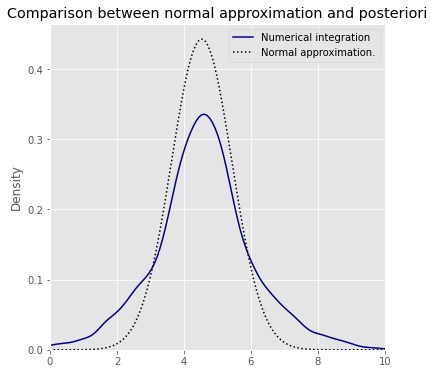
\includegraphics[width=0.5\textwidth]{../../images/comparison-simple-case.png}
    \caption{Posterior density for $\theta$ in Cauchy example and normal approximation.}
    \label{fig:comparison-normal-posteriori}
\end{figure}

\begin{figure}[H]
    \centering
    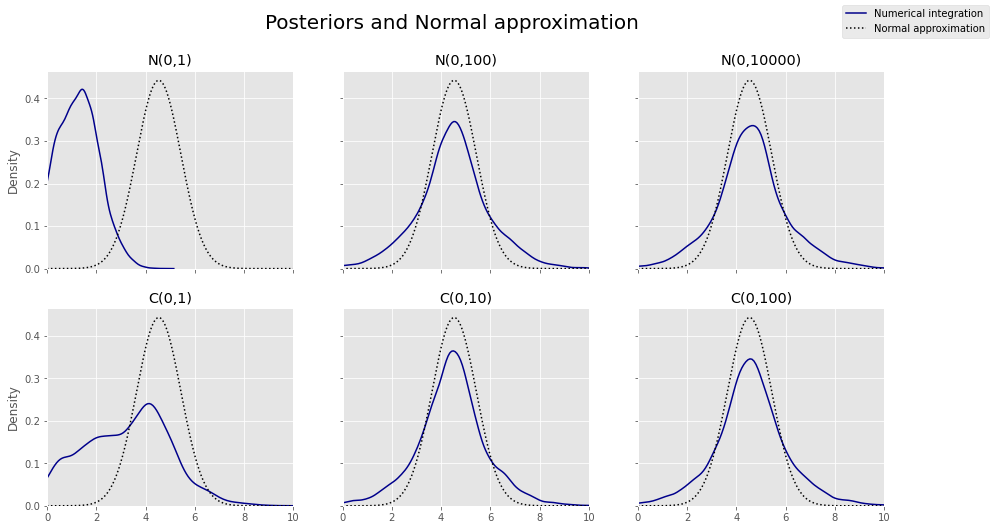
\includegraphics[width=.85\textwidth]{../../images/comparison-other-cases.png}
    \caption{Posterior density for $\theta$ in Cauchy example and normal approximation for other priors.}
    \label{fig:comparison-normal-posteriori-other}
\end{figure}

\section*{Sampling and asymptotic behavior}

We generate samples from Cauchy distribution with location parameter 5 and
scale parameter 1 with sizes specified previously. After that, the parameters of
the Normal distribution are calculated using the principles highted in MLE and
normal approximation sections. They can be visualized in Table
\ref{tb:approximation-normal-sizes}. We see that there is a consistency in the
MLE observed because it seems to converge to 5, what is a good news. The scale
parameter is vanishing apparently. 

\begin{table}[ht]
    \centering
    \begin{tabular}{|c|c|c|c|c|c|c|}
    \hline
    \textbf{Parameter/n} & \textbf{20} & \textbf{50} & \textbf{100} & \textbf{500} & \textbf{1000} & \textbf{10000} \\ \hline
    \textbf{Location}    & 5,4         & 4,67        & 5,05         & 4,98         & 5,01          & 5              \\ \hline
    \textbf{Scale}       & 0,38        & 0,21        & 0,14          & 0,06         & 0,04        & 0,01          \\ \hline
    \end{tabular}
    \caption{Parameters of the normal approximation calculated with precision two.}
    \label{tb:approximation-normal-sizes}
\end{table}

From these values, we can compare the distribution of 
$$
\Sigma_n^{-1/2}(\theta - \hat{\theta}(\bx))
$$
given $X = \bx$ to the Normal distribution with mean 0 and variance 1. We
do not compare the posterior distribution of $\theta$ directly, because we know the
posterior tightens on the true value. We use the Flat prior because it seems to be the chosen by Schervish in the example. We will test the other
prior distributions posteriorly. The results are showed in Figure
\ref{fig:normal-posterior-larger} and they appear to be very interesting.
Even when $n = 20$, we obtain a good approximation. 

\begin{figure}[H]
    \centering
    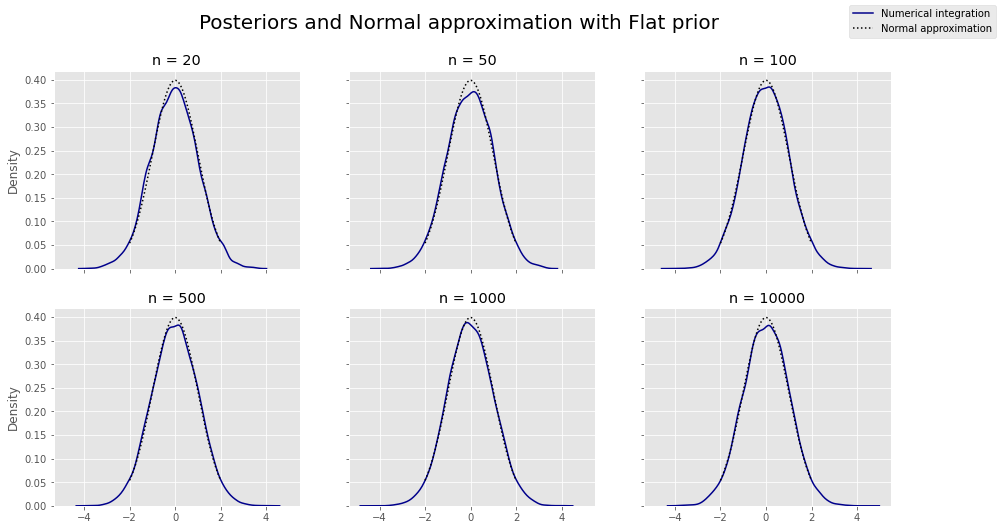
\includegraphics[width=.85\textwidth]{../../images/normal-approximation-large-sample.png}
    \caption{Posterior density for $\theta$ in Cauchy example and normal approximation for larger samples.}
    \label{fig:normal-posterior-larger}
\end{figure}

\newpage

\bibliographystyle{apalike}
\bibliography{bibliography}
\end{document}          
